\documentclass[12pt,a4paper]{article}
\usepackage[utf8]{inputenc} % inutile avec XeLaTeX/LuaLaTeX
\usepackage[T1]{fontenc}
\usepackage{amsmath,amssymb,mathrsfs,tikz,times,pifont}
\usepackage{enumitem}
\usepackage{multicol}
\usepackage{lmodern}
\newcommand\circitem[1]{%
\tikz[baseline=(char.base)]{
\node[circle,draw=gray, fill=red!55,
minimum size=1.2em,inner sep=0] (char) {#1};}}
\newcommand\boxitem[1]{%
\tikz[baseline=(char.base)]{
\node[fill=cyan,
minimum size=1.2em,inner sep=0] (char) {#1};}}
\setlist[enumerate,1]{label=\protect\circitem{\arabic*}}
\setlist[enumerate,2]{label=\protect\boxitem{\alph*}}
\everymath{\displaystyle}
\usepackage[left=1cm,right=1cm,top=1cm,bottom=1.7cm]{geometry}
\usepackage[colorlinks=true, linkcolor=blue, urlcolor=blue, citecolor=blue]{hyperref}
\usepackage{array,multirow}
\usepackage[most]{tcolorbox}
\usepackage{varwidth}
\usepackage{float}
\tcbuselibrary{skins,hooks}
\usetikzlibrary{patterns}

\newtcolorbox{exa}[2][]{enhanced,breakable,before skip=2mm,after skip=5mm,
colback=yellow!20!white,colframe=black!20!blue,boxrule=0.5mm,
attach boxed title to top left ={xshift=0.6cm,yshift*=1mm-\tcboxedtitleheight},
fonttitle=\bfseries,
title={#2},#1,
boxed title style={frame code={
\path[fill=tcbcolback!30!black]
([yshift=-1mm,xshift=-1mm]frame.north west)
arc[start angle=0,end angle=180,radius=1mm]
([yshift=-1mm,xshift=1mm]frame.north east)
arc[start angle=180,end angle=0,radius=1mm];
\path[left color=tcbcolback!60!black,right color = tcbcolback!60!black,
middle color = tcbcolback!80!black]
([xshift=-2mm]frame.north west) -- ([xshift=2mm]frame.north east)
[rounded corners=1mm]-- ([xshift=1mm,yshift=-1mm]frame.north east)
-- (frame.south east) -- (frame.south west)
-- ([xshift=-1mm,yshift=-1mm]frame.north west)
[sharp corners]-- cycle;
},interior engine=empty,
},interior style={top color=yellow!5}}

\usepackage{fancyhdr}
\usepackage{eso-pic}
\usepackage{tkz-tab}
\AddToShipoutPicture{
    \AtTextCenter{%
        \makebox[0pt]{\rotatebox{80}{\textcolor[gray]{0.7}{\fontsize{5cm}{5cm}\selectfont PGB}}}
    }
}

\usepackage{verbatim}

\usepackage{color,soul}

\usepackage{amsmath}
\usepackage{amsfonts}
\usepackage{amssymb}
\usepackage{systeme}
\usepackage{tkz-tab}
\usepackage{tikz}
\usetikzlibrary{arrows}
\newcounter{exemple} % Compteur pour les questions

% Définir la commande pour afficher une question numérotée
\newcommand{\exemple}{%
  \refstepcounter{exemple}%
  \textbf{\textcolor{green}{Exemple \theexemple :}} \ignorespaces
}
%---------------------------------------
\definecolor{myorange}{rgb}{1.0, 0.8, 0.0}

% Définir un compteur pour les exercices d'application
\newcounter{exerciceapp}

% Définir la commande pour afficher un exercice d'application numéroté
\newcommand{\exerciceapp}{%
  \refstepcounter{exerciceapp}%
  \textbf{\textcolor{myorange}{Exercice d'application \theexerciceapp :}} \ignorespaces
}
%--------------------------------------
% Définir un compteur pour les exercices d'application
\newcounter{correction}

% Définir la commande pour afficher un correction exercice d'application numéroté
\newcommand{\correction}{%
  \refstepcounter{correction}%
  \textbf{\textcolor{myorange}{Correction \thecorrection :}} \ignorespaces
}
%--------------------------------------
% Commande pour ajouter du texte en arrière-plan
\usepackage{fancyhdr}
\usepackage{eso-pic}
%\usepackage{tkz-tab}
\AddToShipoutPicture{
    \AtTextCenter{%
        \makebox[0pt]{\rotatebox{80}{\textcolor[gray]{0.7}{\fontsize{5cm}{5cm}\selectfont PGB}}}
    }
}
%This command takes a colour as an optional argument; the default colour is black.
\usetikzlibrary{shapes.geometric,fit}
\newcommand{\myul}[2][black]{\setulcolor{#1}\ul{#2}\setulcolor{black}}
\newcommand\tab[1][1cm]{\hspace*{#1}}

\begin{document}
% En-tête personnalisée
\begin{center}
    \Large\textbf{\underline{\textcolor{red}{Similitude plane directe}}}\\[-0.1cm]
    \normalsize\textbf{Prof : M. BA} \hfill \textbf{Classe : TS2}\\[-0.1cm]
    \textbf{Année scolaire : 2024 -- 2025}
\end{center}


\section*{\underline{I) Complexe et transformation du plan}}

\subsection*{\underline{1) Fonction dans $\mathbb{C}$ associée à une transformation du plan}}

\noindent
\begin{minipage}{0.5\textwidth}
    Soit $f : \mathbb{C} \to \mathbb{C}$
    \[ z \to f(z) \]
\end{minipage}
\begin{minipage}{0.5\textwidth}
    \raggedleft
    Soit $F : \mathcal{P} \to \mathcal{P}$ \hspace{3em}
    \[ M(z) \to M'(z') \]
\end{minipage}

\vspace{1em}

\noindent \textbf{Si $f$ est une bijection de $\mathbb{C}$ dans $\mathbb{C}$, alors}

\vspace{1em}

\noindent \textbf{$F$ est la transformation du plan associée à la bijection complexe $f$ dans $\mathbb{C}$.}

\subsection*{\underline{2) Transformations élémentaires du plan}}

\noindent \textbf{Soient M, N, P et Q les points d'affixes respectives $z$, $\bar{z}$, $-z$ et $-\bar{z}$.}

\vspace{1em}

% Reproduction du graphique avec TikZ
\begin{center}
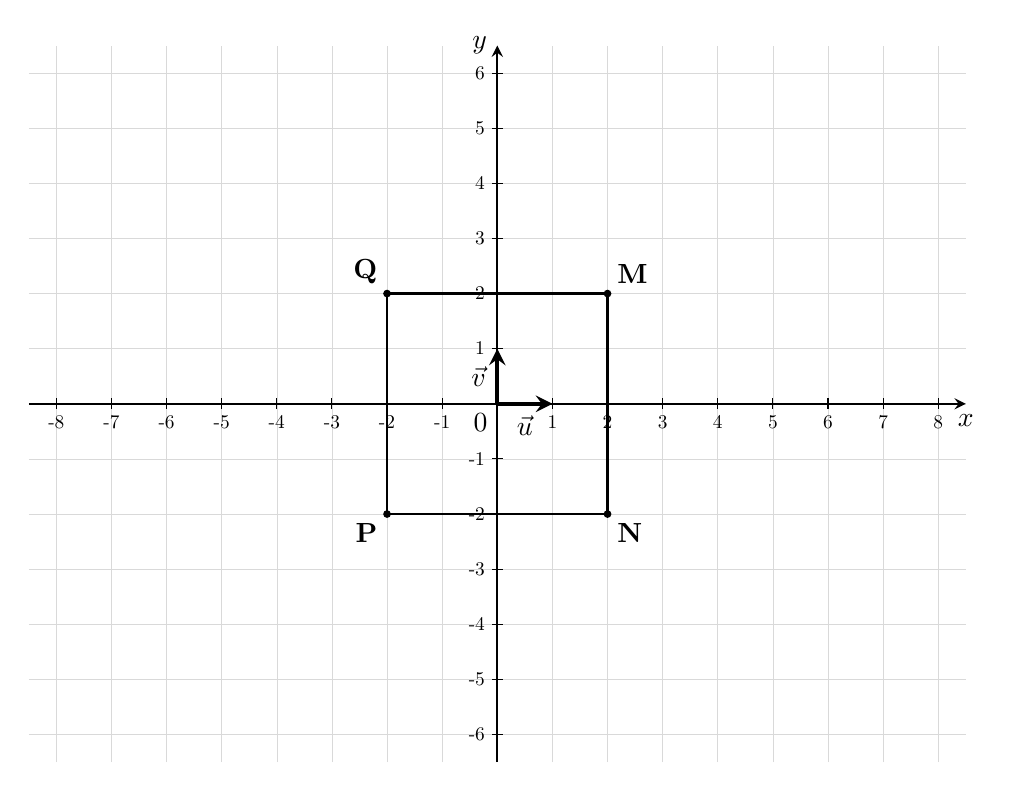
\begin{tikzpicture}[scale=0.7, >=stealth]
    % Grille et axes
    \draw[very thin, gray!30] (-8.5,-6.5) grid (8.5,6.5);
    \draw[->, thick] (-8.5,0) -- (8.5,0) node[below] {$x$};
    \draw[->, thick] (0,-6.5) -- (0,6.5) node[left] {$y$};
    
    % Graduations
    \foreach \x in {-8,-7,...,-1,1,2,...,8}
        \draw (\x, 0.1) -- (\x, -0.1) node[below, scale=0.7] {\x};
    \foreach \y in {-6,-5,...,-1,1,2,...,6}
        \draw (0.1, \y) -- (-0.1, \y) node[left, scale=0.7] {\y};
    \node[below left] at (0,0) {0};

    % Vecteurs unitaires
    \draw[->, ultra thick] (0,0) -- (1,0) node[midway, below] {$\vec{u}$};
    \draw[->, ultra thick] (0,0) -- (0,1) node[midway, left] {$\vec{v}$};

    % Points et rectangle
    \coordinate (M) at (2,2);
    \coordinate (N) at (2,-2);
    \coordinate (P) at (-2,-2);
    \coordinate (Q) at (-2,2);

    \draw[thick] (M) -- (N) -- (P) -- (Q) -- cycle;

    \fill (M) circle (2pt) node[above right] {\textbf{M}};
    \fill (N) circle (2pt) node[below right] {\textbf{N}};
    \fill (P) circle (2pt) node[below left] {\textbf{P}};
    \fill (Q) circle (2pt) node[above left] {\textbf{Q}};
\end{tikzpicture}
\end{center}

\vspace{1em}

\begin{itemize}
    \item[$\bullet$] \textit{\textbf{La symétrie d'axe(OI) a pour écriture complexe $z' = \bar{z}$.}}
    \item[$\bullet$] \textit{\textbf{La symétrie d'axe(OJ) a pour écriture complexe $z' = -\bar{z}$.}}
    \item[$\bullet$] \textit{\textbf{La symétrie de centre O a pour écriture complexe $z' = -z$.}}
\end{itemize}

\subsection*{\underline{3) Translation}}

\noindent \textbf{Toute transformation du plan d'écriture complexe $z' = z + b$, $b \in \mathbb{C}$, est une translation de vecteur $\vec{u}$ d'affixe $b$.}

\vspace{0.5em}
\noindent \colorbox{blue!20}{\textbf{\textit{Démonstration}}}
\vspace{1em}

\begin{center}
    $t_{\vec{u}} : \mathcal{P} \to \mathcal{P}$ \\
    $M(z) \to t_{\vec{u}}(M) = M'(z')$
\end{center}

\noindent $t_{\vec{u}}(M) = M' \quad \iff \quad \vec{u} = \vec{MM'} \quad \iff \quad z_{\vec{u}} = z_{\vec{MM'}}$

\vspace{1em}

\noindent $z_{\vec{u}} = z_{\vec{MM'}} = z_{M'} - z_{M} \cdot z_{\vec{u}} = z_{M'} - z_{M}$. Or $z_{M'} = z'$, $z_{M} = z$.

\vspace{1em}

\noindent On pose : $z_{\vec{u}} = b$.

\vspace{1em}

\noindent On obtient : $b = z' - z \quad$ d'où $\quad z' = z + b$.

\vspace{1em}

\noindent \textbf{Toute écriture complexe de la forme : $z' = z + b$ est une translation de vecteur $\vec{u}$ d'affixe $b$.}

\noindent \colorbox{blue!20}{\textbf{\textit{Exercice d'application}}}

\vspace{1em}

\noindent 1) Donner la nature de la transformation du plan d'écriture complexe : $z' = z - 3 + 2i$.

\noindent 2) Soit la translation de vecteur $\vec{u}$ d'affixe $-2 + i$. Donner son écriture complexe.

\vspace{1em}

\noindent \colorbox{blue!20}{\textbf{\textit{Solution}}}

\vspace{1em}

\noindent 1) Donnons la nature de la transformation du plan d'écriture complexe : $z' = z - 3 + 2i$.

\noindent : $z' = z - 3 + 2i \quad , \quad b = -3 + 2i$.

\vspace{1em}

\noindent \fbox{\textbf{La transformation du plan est la translation de vecteur $\vec{u}$ d'affixe $-3 + 2i$.}}

\vspace{1em}

\noindent 2) Soit la translation de vecteur $\vec{u}$ d'affixe $-2 + i$. Donnons son écriture complexe.

\noindent Le vecteur $\vec{u}$ est d'affixe $-2 + i$ donc $b = -2 + i$.

\vspace{1em}

\noindent \fbox{\textbf{La translation de vecteur $\vec{u}$ d'affixe $-2 + i$ est d'écriture complexe : $z' = z - 2 + i$.}}

\section*{4) \underline{Homothétie}}

\noindent \textbf{Toute transformation du plan d'écriture complexe $z' = az + b$, $a \in \mathbb{R} \setminus \{0; 1\}$, $b \in \mathbb{C}$, est une homothétie de rapport $k = a$ et de centre $\Omega$ tel que $z_{\Omega} = \frac{b}{1 - a}$.}

\vspace{1em}

\noindent \colorbox{blue!20}{\textbf{\textit{Démonstration}}}

\begin{center}
$
\begin{aligned}
h(\Omega, k) :& \mathcal{P}& \to \mathcal{P} \\
&M(z)& \to h(\Omega, k)(M) = M'(z')
\end{aligned}
$
\end{center}

\noindent $h(\Omega, k)(M) = M' \quad \iff \quad \overrightarrow{\Omega M'} = k \overrightarrow{\Omega M} \quad \iff \quad z_{\overrightarrow{\Omega M'}} = z_{k \overrightarrow{\Omega M}}$

\vspace{1em}

\noindent $z_{\overrightarrow{\Omega M'}} = z_{k \overrightarrow{\Omega M}} = k z_{\overrightarrow{\Omega M}} \quad \iff \quad z_{M'} - z_{\Omega} = k(z_M - z_{\Omega})$. Or $z_{M'} = z'$, $z_M = z$.

\vspace{1em}

\noindent On obtient : $z' - z_{\Omega} = k(z - z_{\Omega})$, \quad $z' - z_{\Omega} = kz - kz_{\Omega}$ \quad donc $z' = kz + (1 - k) z_{\Omega}$.

\vspace{1em}

\noindent Posons $k = a$ \quad et \quad $b = (1 - k) z_{\Omega}$ \quad donc $z' = az + b$.

\vspace{1em}

\noindent $k = a$ \quad donc $b = (1 - a) z_{\Omega}$ \quad donc \quad $z_{\Omega} = \frac{b}{1 - a}$.

\vspace{1em}

\noindent \textbf{Toute transformation du plan d'écriture complexe $z' = az + b$, $a \in \mathbb{R} \setminus \{0; 1\}$, $b \in \mathbb{C}$, est une homothétie de rapport $k = a$ et de centre $\Omega$ tel que $z_{\Omega} = \frac{b}{1 - a}$.}

\end{document}